\chapter{Background}

In this chapter I am going to introduce the reader to the concepts that are necessary to understand the research presented in this thesis. The chapter is divided into three sections. The first section provides an overview of Variational Autoencoders (VAEs) and their applications. The second section introduces Vector Quantized VAEs (VQ-VAEs). The third section introduces Multitask VAEs (MT-VAEs), which are the main focus of this thesis.

\section{VAEs}

Variational Autoencoders (VAEs), first introduced in 2013 by Kingma and Welling\cite{kingma2022autoencoding}, have become a prominent class of generative models in the field of machine learning.  At their core, VAEs consist of an encoder network with parameters $\phi$ that maps data points $x$ into a latent space $z$ and a decoder network with parameters $\theta$ that generates data $\hat{x}$ from latent representations\cite{Kingma_2019}. 

The key innovation that makes VAEs work is the introduction of a probabilistic interpretation of the latent space. More specifically, VAEs assume that the latent space $z$ is a random variable that follows a certain prior distribution $p(z)$, which is typically a Gaussian distribution and that the mapping from the latent space to the data space is also probabilistic\cite{kingma2022autoencoding}.

The optimization target for VAEs is the evidence lower bound (ELBO) which is: \[ L_{\theta, \phi}(x) = \mathbb{E}_{q_{\phi}(z|x)} [\log p_{\theta}(x, z) - \log q_{\phi}(z|x)] \] where $q_{\phi}(z|x)$ is the encoder distribution, $p_{\theta}(z, x)$ is the decoder distribution and $p(z)$ is the prior distribution. The individual datapoint ELBO and its gradient is, in general, intractable. However, this is where reparametrization trick comes which is discussed in the next section.

The ELBO can be also written as a sum of two terms\cite{kingma2022autoencoding}
: \[ L_{\theta, \phi}(x) = \mathbb{E}_{q_{\phi}(z|x)} [\log p_{\theta}(x|z)] - D_{KL}(q_{\phi}(z|x) || p(z)) \] where the first term is the reconstruction loss and the second term is the regularization term. The first term is the negative reconstruction loss, which is the negative log-likelihood of the data given the latent representation. The second term is the Kullback-Leibler divergence between the encoder distribution and the prior distribution. The Kullback-Leibler divergence is a measure of how much one probability distribution differs from another probability distribution. In this case, it is a measure of how much the encoder distribution differs from the prior distribution. The Kullback-Leibler divergence is always non-negative, so minimizing the Kullback-Leibler divergence is equivalent to maximizing the ELBO.
\subsection{Reparametrization Trick}

The Reparametrization trick also  is a crucial component of VAEs. It is used to make the ELBO differentiable w.r.t the parameters of the encoder $\phi$ and decoder $\theta$. The notion is based on the fact we can define a random variable $z \sim q_{\phi}(z|x)$ as a deterministic function of a random variable $\epsilon$ and the parameters $\phi$ such that $z = g_{\phi}(\epsilon, x)$, where the distribution of $\epsilon$ is independent of $\phi$ and $x$: $\epsilon \sim p(\epsilon)$. With this parameterization, the expectation w.r.t $q_{\phi}(z|x)$ can be rewritten as an expectation w.r.t. $p(\epsilon)$: \[ L_{\theta, \phi}(x) = \mathbb{E}_{q_{\phi}(z|x)} [\log p_{\theta}(x, z) - \log q_{\phi}(z|x)] \]
\[ = \mathbb{E}_{p(\epsilon)} [\log p_{\theta}(x, g_{\phi}(\epsilon, x)) - \log q_{\phi}(g_{\phi}(\epsilon, x)|x)] \] which is differentiable w.r.t $\phi$ and $\theta$.

\subsection{Implementation}

In a standard VAE implementation we have an analytical solution 

\begin{figure}[H]
    \centering
    \makebox[\textwidth]{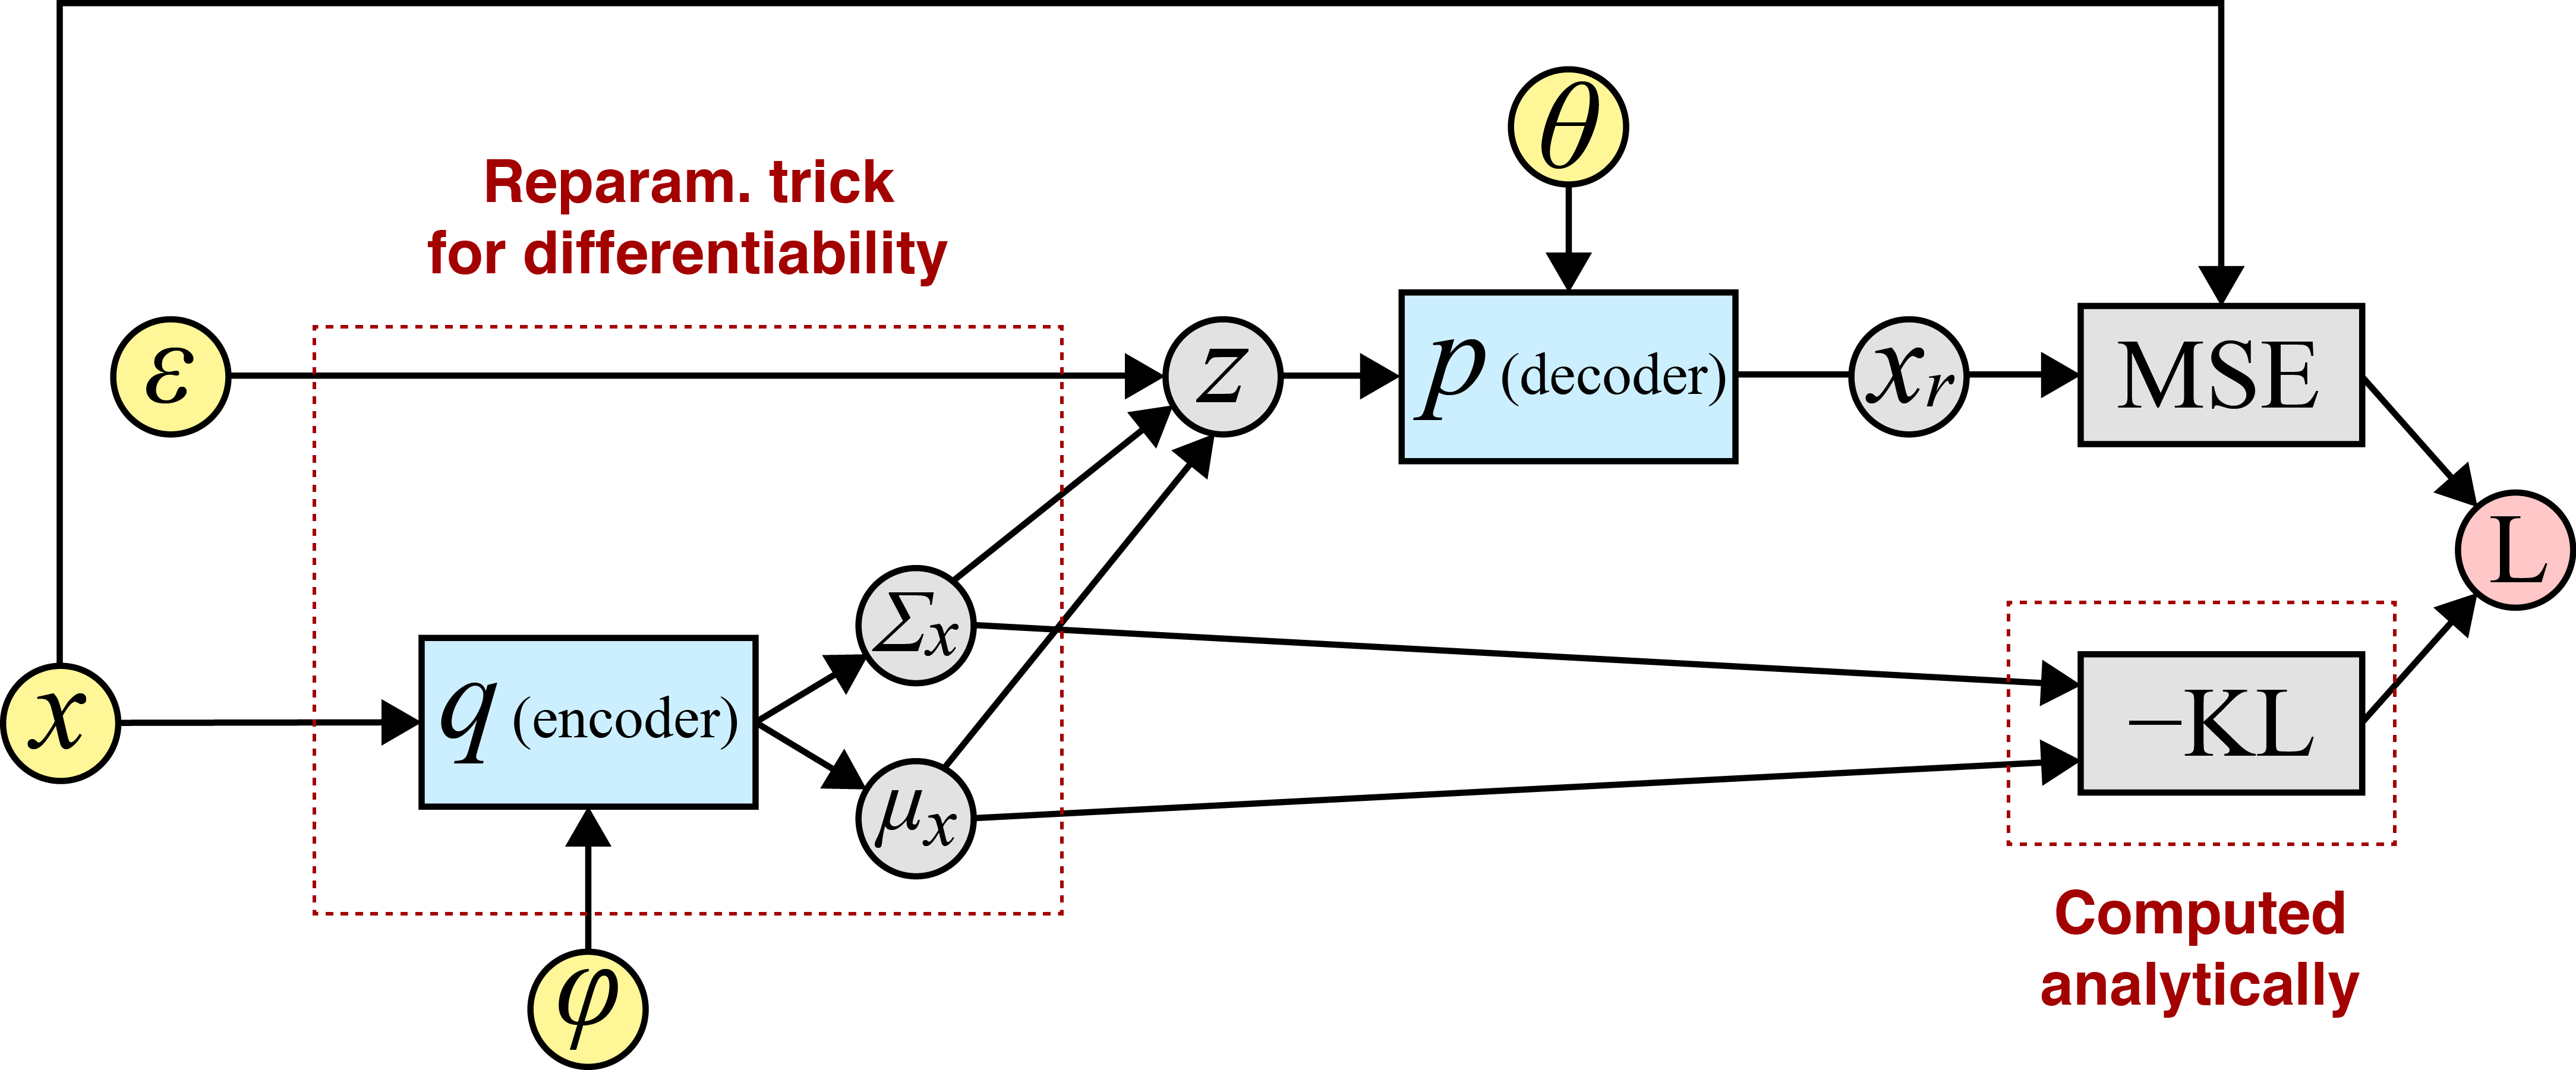
\includegraphics[width=\textwidth]{figures/vae}}

    \caption{ The architecture of VAEs.}
  	\medskip 
	\hspace*{15pt}\hbox{\scriptsize Credit: Aäron van den Oord et al.}
    \label{VAEFigure}

\end{figure}

\section{Vector Quantized VAEs}

Vector Quantized VAEs (VQ-VAEs) are a variant of VAEs that were introduced in 2017 by Aäron van den Oord et al\cite{vqvae}. VQ-VAEs successfully combine the VAE framework with discrete latent representations using a technique called Vector Quantization. 

\begin{figure}[H]
    \centering
    \makebox[\textwidth]{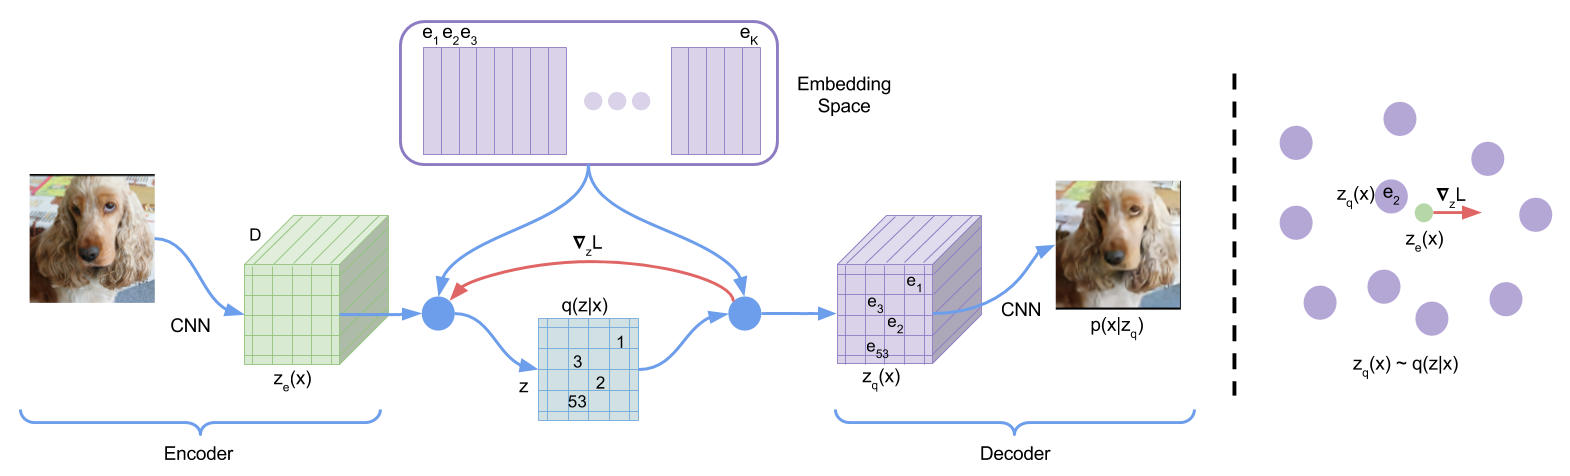
\includegraphics[width=\textwidth]{figures/vq_vae}}

    \caption{On the left side there is a figure describing the VQ-VAE architecture. On the right side there is visualization of the latent space whilst training. The figure is taken from \cite{vqvae}.}
  	\medskip 
	\hspace*{15pt}\hbox{\scriptsize Credit: Aäron van den Oord et al.}
    \label{VQVAEFigure}

\end{figure}
